\newpage
\section{Exercises}

These exercises are intended to get you started with programming with
\emph{\index{Python}{Python}} and the \emph{\index{NumPy}{NumPy}} and
Matplotlib libraries. If you are already familiar with these topics,
you may want to skip these exercises.

\begin{enumerate}
 \item Obtain the source code for the examples by cloning the github
   repository for this course. 
\item The Hello World program shown in Listing \ref{lst:pythonhw} plots a complex sinusoidal signal. 
  \begin{enumerate}[a)]
  \item Go on the NumPy web site \url{http://numpy.org}, and find the documentation the functions included in the package.
  \item Use this documentation to determine what \verb|numpy.arange|, and \verb|numpy.exp| do. 
  \item Modify the code so that it plots a circle on the complex
    plane, by plotting the real part of the complex sinusoidal
    signal \verb|csin| on the x-axis, and the imaginary part on the
    y-axis.
  \item Explain why the real and imaginary component draw a circle on the complex plane.
  \end{enumerate}

\item Use Python to calculate and print out the value of $e^{i \pi} + 1$. Note that $i$ in Python is denoted
  with \verb|1j|.
  
\item The use of built-in Numpy functions will let you program
  efficiently. The program shown in Listing \ref{lst:exercise002}
  demonstrates the use of Numpy functions to evaluate the Mandelbrot
  set with a slight twist.

\lstinputlisting[language=Python,caption={\texttt{001\_hello\_world/mystery.py}},label=lst:exercise002]{code/001_hello_world/mystery.py}

\begin{enumerate}[a)]
  \item Run the program shown in Listing \ref{lst:exercise002}. You
    	should see a plot like the one shown in Figure \ref{fig:mandelbrot}.
  \item Describe what each line of the program does by adding comments to the code.
  \item It is possible to specify the data type of a NumPy array
      	using the \verb|dtype| attribute? There are two complex valued
      	datatypes available in NumPy: \verb|complex64| and \verb|complex128|. 
      	What are to pros and cons of using the \verb|complex64| datatype 
      	instead of the \verb|complex128| datatype? 
\end{enumerate}


\begin{figure}
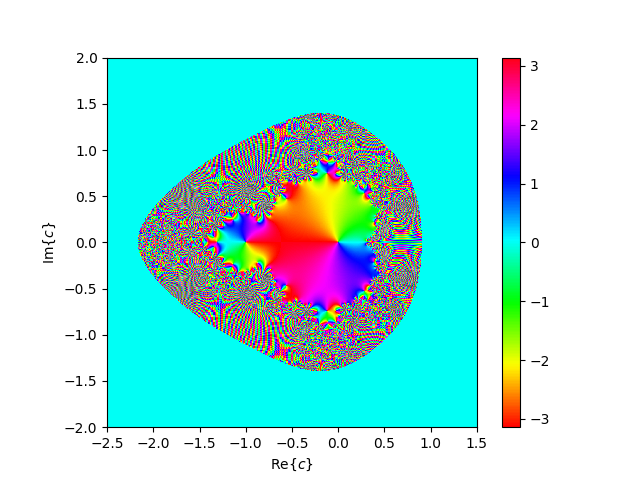
\includegraphics[width=0.9\textwidth]{ch02/figures/mystery.png}
\caption{The Mandelbrot set example demonstrates the use of NumPy array functions and complex numbers. The plots
  shows the phase of complex number $z_{12}$ after 12 iterations of
  $z_{n+1} \leftarrow z_n^2 + c$, starting with $z_0 = 0$.}
\label{fig:mandelbrot}
\end{figure}



\end{enumerate}
